\documentclass[11pt,letter]{article}

\usepackage[utf8]{inputenc}
\usepackage{latexsym}
\usepackage{amsmath}
\usepackage{graphicx}
\usepackage{tikz-dependency}
\usepackage{natbib}
\bibpunct{(}{)}{,}{a}{}{;}

\setlength{\textwidth}{16cm}
\setlength{\oddsidemargin}{-0.04cm}
\setlength{\topmargin}{-2cm}
\setlength{\textheight}{23.5cm}

\newcommand{\mystretch}{1.1}
\renewcommand{\baselinestretch}{\mystretch}

\def\url#1{\textsf{#1}}


\title{\textbf{Stanford typed dependencies manual}}
\author{Marie-Catherine de Marneffe and Christopher D. Manning}
\date{September 2008\\
%Revised for Stanford Parser v. 1.6.2 in February 2010
%Revised for Stanford Parser v.~1.6.5 in November 2010
%Revised for Stanford Parser v.\ 1.6.9 in September 2011
% Revised for Stanford Parser v.\ 2.0.4 in November 2012
Revised for the Stanford Parser v.\ 2.0.5 in March 2013
}

\begin{document}
\maketitle

\section{Introduction}

The Stanford typed dependencies representation was designed to provide
a simple description of the grammatical relationships in a sentence
that can easily be understood and effectively used by people without
linguistic expertise who want to extract textual relations.  In
particular, rather than the phrase structure representations that have
long dominated in the computational linguistic community, it
represents all sentence relationships uniformly as typed dependency
relations. That is, as triples of a relation between pairs of words, such as ``the subject of
\emph{distributes} is \emph{Bell.}''  Our experience is that this simple,
uniform representation is quite accessible to non-linguists
thinking about tasks involving information extraction from text and is
effective in relation extraction applications.

Here is an example sentence:
\begin{quote}
\emph{Bell, based in Los Angeles, makes and distributes electronic, computer and building products.}
\end{quote}
For this sentence, the Stanford Dependencies (SD) representation is:
\begin{quote}
nsubj(makes-8, Bell-1) \\
nsubj(distributes-10, Bell-1) \\
partmod(Bell-1, based-3) \\
nn(Angeles-6, Los-5) \\
prep\_in(based-3, Angeles-6) \\
root(ROOT-0, makes-8)\\
conj\_and(makes-8, distributes-10) \\
amod(products-16, electronic-11) \\
conj\_and(electronic-11, computer-13) \\
amod(products-16, computer-13) \\
conj\_and(electronic-11, building-15) \\
amod(products-16, building-15) \\
dobj(makes-8, products-16) \\
dobj(distributes-10, products-16)
\end{quote}

These dependencies map straightforwardly onto a directed graph representation, in which words in the sentence are nodes in the graph and grammatical relations are edge labels. Figure~\ref{bell} gives the graph representation for the example sentence above.
\begin{figure}
\begin{center}
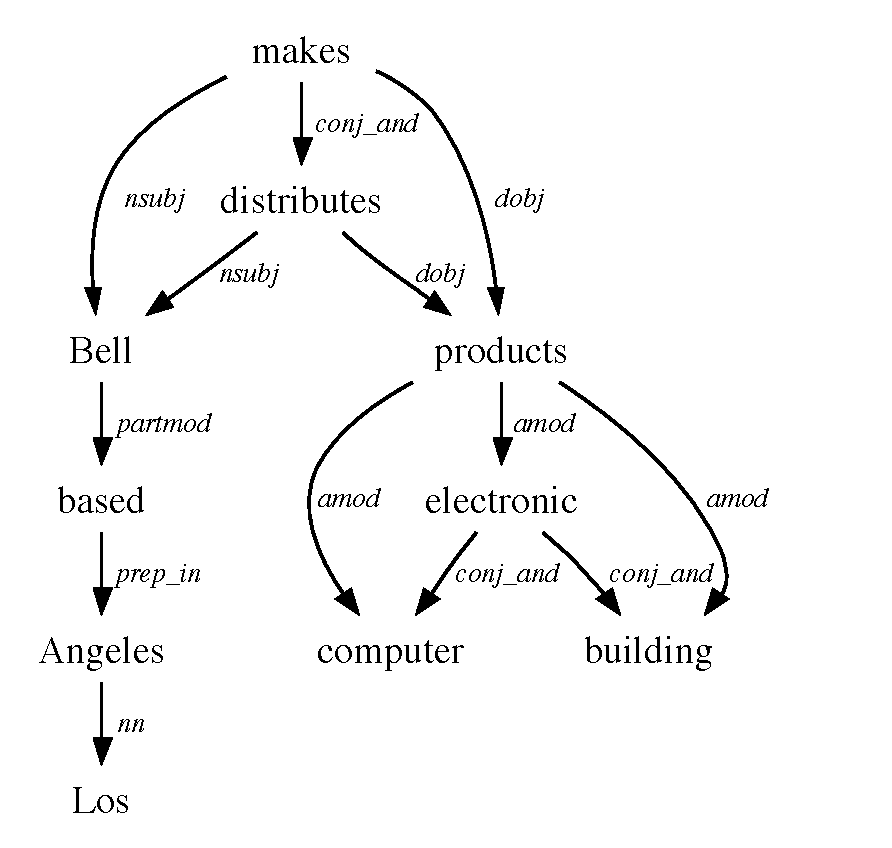
\includegraphics[width=3.2in, height=3.0in]{bell.pdf}
\end{center}
\vspace*{-0.6cm}
\caption{\label{bell} Graphical representation of the Stanford Dependencies for the sentence: \emph{Bell, based in Los Angeles, makes and distributes electronic, computer and building products.}}
\end{figure}

\subparagraph{Document overview:} This manual provides documentation about the set of dependencies defined
for English.  (There is also a Stanford Dependency representation
available for Chinese, but it is not further discussed here.)  Section~\ref{def}
of the manual defines the relations and the taxonomic hierarchy over
them appears in section~\ref{hierarchy}.  This is then followed by a description of the several variant
dependency representations available, aimed at different use cases
(section~\ref{types}), some details of the software available for
generating Stanford Dependencies (section~\ref{in_practice}), and
references to further discussion and use of the SD representation (section~\ref{refs}).


\section{Definitions of the Stanford typed dependencies}\label{def}

The current representation contains approximately 50 grammatical
relations (depending slightly on the options discussed in section~\ref{types}). The dependencies are all binary relations: a grammatical relation holds between a \emph{governor} (also known as a \emph{regent} or a \emph{head}) and a dependent. The grammatical relations are defined below, in alphabetical order according to the dependency's abbreviated name (which appears in the parser output). The definitions make use of the Penn Treebank part-of-speech tags and phrasal labels.

\bigskip

\noindent\textbf{\emph{acomp}: adjectival complement}\\
An adjectival complement of a verb is an adjectival phrase which functions as the complement (like an object of the verb).
\begin{tabbing}
\hspace{1cm} \=XXXXXXXXXXXXXXXXXXXXXXXXXXXX\= \hspace{1cm}\=  \kill
\> ``She looks very beautiful" \>\> \emph{acomp}(looks, beautiful)\\
\end{tabbing}

\noindent\textbf{\emph{advcl}: adverbial clause modifier}\\
An adverbial clause modifier of a VP or S is a clause modifying the
verb (temporal clause, consequence, conditional clause, purpose
clause, etc.).
\begin{tabbing}
	\hspace{1cm} \=XXXXXXXXXXXXXXXXXXXXXXXXXXXX\= \hspace{1cm}\=  \kill
\> ``The accident happened as the night was falling" \> \> \emph{advcl}(happened, falling)\\
\> ``If you know who did it, you should tell the teacher" \> \> \emph{advcl}(tell, know)\\
\> ``He talked to him in order to secure the account" \>  \> \emph{advcl}(talked, secure)\\
\end{tabbing}

\noindent\textbf{\emph{advmod}: adverbial modifier}\\
An adverbial modifier of a word is a (non-clausal) adverb or adverbial phrase (ADVP) that serves to modify the meaning of the word.
\begin{tabbing}
\hspace{1cm} \=XXXXXXXXXXXXXXXXXXXXXXXXXXXX\= \hspace{1cm}\=  \kill
\>  ``Genetically modified food" \> \> \emph{advmod}(modified, genetically)\\
\> ``less often" \> \> \emph{advmod}(often, less)\\
\end{tabbing}

\noindent\textbf{\emph{agent}: agent}\\
An agent is the complement of a passive verb which is introduced by the preposition ``by" and does the action.
This relation only appears in the collapsed dependencies, where it can
replace \emph{prep\_by}, where appropriate. It does not appear in
basic dependencies output.
\begin{tabbing}
\hspace{1cm} \=XXXXXXXXXXXXXXXXXXXXXXXXXXXX\= \hspace{1cm}\=  \kill
\>  ``The man has been killed by the police" \> \> \emph{agent}(killed, police)\\
\> ``Effects caused by the protein are important'' \> \> \emph{agent}(caused, protein)\\
\end{tabbing}

\noindent\textbf{\emph{amod}: adjectival modifier}\\
An adjectival modifier of an NP is any adjectival phrase that serves to modify the meaning of the NP.
\begin{tabbing}
\hspace{1cm} \= xxxxxxxxxxxxxxxxxxxxxxxxxx\= \hspace{.5cm}\=  \kill
\> ``Sam eats red meat" \> \> \emph{amod}(meat, red)\\
\end{tabbing}

\noindent\textbf{\emph{appos}: appositional modifier}\\
An appositional modifier of an NP is an NP immediately to the right of
the first NP that serves to define or modify that NP. It includes
parenthesized examples, as well as defining abbreviations in one of
these structures
\begin{quote}
\begin{dependency}
   \begin{deptext}[column sep=0.2em]
      Sam \&, \& my \& brother \& , \& arrived \\
   \end{deptext}
   \depedge[edge unit distance=0.5ex]{1}{4}{appos}
\end{dependency}
\hspace*{1in}
\begin{dependency}
   \begin{deptext}[column sep=0.2em]
      Bill\& ( \& John \& 's \& cousin \& ) \\
   \end{deptext}
   \depedge[edge unit distance=0.5ex]{1}{5}{appos}
\end{dependency}

\begin{dependency}
   \begin{deptext}[column sep=0.2em]
      The \& Australian \& Broadcasting \& Corporation \& ( \& ABC \& ) \\
   \end{deptext}
   \depedge[edge unit distance=1ex]{4}{6}{appos}
\end{dependency}
\end{quote}

\noindent\textbf{\emph{attr}: attributive}\\
An attributive is a complement of a copular verb such as ``to be", ``to seem", ``to appear". Currently, the converter only recognizes WHNP complements.
\begin{tabbing}
\hspace{1cm} \= xxxxxxxxxxxxxxxxxxxxxxxxxx\= \hspace{.5cm}\=  \kill
\>  ``What is that?" \> \>  \emph{attr}(is, What)\\
\end{tabbing}

\noindent \textbf{\emph{aux}: auxiliary}\\
An auxiliary of a clause is a non-main verb of the clause, e.g.\@ modal auxiliary, ``be" and ``have" in a composed tense.
\begin{quote}
\begin{dependency}
   \begin{deptext}[column sep=0.25cm]
      Reagan \& has \& died \\
   \end{deptext}
   \depedge{3}{2}{aux}
\end{dependency}
\hspace*{1in}
\begin{dependency}
   \begin{deptext}[column sep=0.25cm]
      He \& should \& leave \\
   \end{deptext}
   \depedge{3}{2}{aux}
\end{dependency}
\end{quote}

\noindent \textbf{\emph{auxpass}: passive auxiliary}\\
A passive auxiliary of a clause is a non-main verb of the clause which contains the passive information.
\begin{tabbing}
\hspace{1cm} \= xxxxxxxxxxxxxxxxxxxxxxxxxx\= \hspace{.5cm}\=  \kill
\> ``Kennedy has been killed"  \> \> \emph{auxpass}(killed, been)\\
\> \> \> \emph{aux}(killed,has)\\
\> ``Kennedy was/got killed'' \> \> \emph{auxpass}(killed, was/got)\\
\end{tabbing}

\noindent\textbf{\emph{cc}: coordination}\\
A coordination is the relation between an element of a conjunct and the coordinating conjunction word of the conjunct.  (Note: different dependency grammars have different treatments of coordination.  We take one conjunct of a conjunction (normally the first) as the head of the conjunction.)
A conjunction may also appear at the beginning of a sentence.  This is also called a cc, and dependent on the root predicate of the sentence.
\begin{tabbing}
\hspace{1cm} \= xxxxxxxxxxxxxxxxxxxxxxxxxx\= \hspace{.5cm}\=  \kill
\>  ``Bill is big and honest" \hspace{1cm} \> \> \emph{cc}(big, and)\\
\hspace{1cm} \> ``They either ski or snowboard" \> \> \emph{cc}(ski, or)\\
\> ``And then we left.'' \> \> \emph{cc}(left, And)\\
\end{tabbing}

\noindent\textbf{\emph{ccomp}: clausal complement}\\
A clausal complement of a verb or adjective is a dependent clause with an internal subject which functions like an object of the verb, or adjective.  Clausal complements for nouns are limited to complement clauses with a subset of nouns
 like ``fact'' or ``report''.  We analyze them the same (parallel to the
 analysis of this class as ``content clauses'' in Huddleston and Pullum 2002). Such clausal complements are usually finite (though there are occasional remnant English subjunctives).
\begin{tabbing}
\hspace{1cm} \= xxxxxxxxxxxxxxxxxxxxxxxxxxxxxxxx\= \hspace{.5cm}\=  \kill
\>  ``He says that you like to swim" \> \> \emph{ccomp}(says, like)\\
\hspace{1cm} \> ``I am certain that he did it" \> \>  \emph{ccomp}(certain, did)\\
\hspace{1cm} \> ``I admire the fact that you are honest'' \>\> \emph{ccomp}(fact, honest)\\
\end{tabbing}

\noindent\textbf{\emph{conj}: conjunct}\\
A conjunct is the relation between two elements connected by a coordinating conjunction, such as ``and", ``or", etc.  We treat conjunctions asymmetrically: The head of the relation is the first conjunct and other conjunctions depend on it via the \emph{conj} relation.
\begin{tabbing}
\hspace{1cm} \= xxxxxxxxxxxxxxxxxxxxxxxxxx\= \hspace{.5cm}\=  \kill
\>  ``Bill is big and honest" \> \> \emph{conj}(big, honest)\\
\hspace{1cm} \> ``They either ski or snowboard" \> \>  \emph{conj}(ski, snowboard)\\
\end{tabbing}

\noindent\textbf{\emph{cop}: copula}\\
A copula is the relation between the complement of a copular verb and the copular verb.  (We normally take a copula as a dependent of its complement; see the discussion in section~\ref{types}.)
\begin{tabbing}
\hspace{1cm} \= xxxxxxxxxxxxxxxxxxxxxxxxxx\= \hspace{.5cm}\=  \kill
\> ``Bill is big" \hspace{1cm} \> \> \emph{cop}(big, is)\\
\hspace{1cm} \> ``Bill is an honest man" \>  \> \emph{cop}(man, is)\\
\end{tabbing}

\noindent\textbf{\emph{csubj}: clausal subject}\\
A clausal subject is a clausal syntactic subject of a clause, i.e., the subject is itself a clause. The governor of this relation might not always be a verb: when the verb is a copular verb, the root of the clause is the complement of the copular verb. In the two following examples, ``what she said'' is the subject.
\begin{tabbing}
\hspace{1cm} \= xxxxxxxxxxxxxxxxxxxxxxxxxx\= \hspace{.5cm}\=  \kill
\> ``What she said makes sense" \> \> \emph{csubj}(makes, said)\\
\hspace{1cm} \> ``What she said is not true" \> \>  \emph{csubj}(true, said)\\
\end{tabbing}

\noindent\textbf{\emph{csubjpass}: clausal passive subject}\\
A clausal passive subject is a clausal syntactic subject of a passive clause. In the example below, ``that she lied'' is the subject.
\begin{tabbing}
\hspace{1cm} \=XXXXXXXXXXXXXXXXXXXXXXXXXXXX\= \hspace{1cm}\=  \kill
\>  ``That she lied was suspected by everyone" \> \> \emph{csubjpass}(suspected, lied)\\
\end{tabbing}

\noindent\textbf{\emph{dep}: dependent}\\
A dependency is labeled as dep when the system is unable to determine a more precise dependency relation between two words.  This may be because of a weird grammatical construction, a limitation in the Stanford Dependency conversion software, a parser error, or because of an unresolved long distance dependency.
\begin{tabbing}
\hspace{1cm} \= xxxxxxxxxxxxxxxxxxxxxxxxxxxxxxxxxx\= \hspace{.5cm}\=  \kill
\>  ``Then, as if to show that he could, \ldots" \> \> \emph{dep}(show, if)\\
\end{tabbing}

\noindent\textbf{\emph{det}: determiner}\\
A determiner is the relation between the head of an NP and its determiner.
\begin{tabbing}
\hspace{1cm} \= xxxxxxxxxxxxxxxxxxxxxxxxxx\= \hspace{.5cm}\=  \kill
\>  ``The man is here" \> \> \emph{det}(man, the)\\
\> ``Which book do you prefer?" \> \> \emph{det}(book, which)\\
\end{tabbing}

\noindent\textbf{\emph{discourse}: discourse element}\\
This is used for interjections and other discourse particles and
elements (which are not clearly linked to the structure of the
sentence, except in an expressive way). We generally follow the
guidelines of what the Penn Treebanks count as an INTJ.  They
define this to include: interjections (\emph{oh}, \emph{uh-huh},
\emph{Welcome}), fillers (\emph{um}, \emph{ah}), and discourse
markers (\emph{well}, \emph{like}, \emph{actually}, but not \emph{you know}).
\begin{quote}
\begin{dependency}
   \begin{deptext}[column sep=0.25cm]
      Iguazu \& is \& in \& Argentina \& :) \\
   \end{deptext}
   \depedge[edge unit distance=0.4ex]{2}{5}{discourse}
\end{dependency}
\end{quote}

\noindent\textbf{\emph{dobj}: direct object}\\
The direct object of a VP is the noun phrase which is the (accusative) object of the verb.
\begin{tabbing}
\hspace{1cm} \= xxxxxxxxxxxxxxxxxxxxxxxxxx\= \hspace{.5cm}\=  \kill
\>  ``She gave me a raise" \> \> \emph{dobj}(gave, raise)\\
\hspace{1cm} \> ``They win the lottery" \> \>  \emph{dobj}(win, lottery)\\
\end{tabbing}


\noindent\textbf{\emph{expl}: expletive}\\
This relation captures an existential ``there". The main verb of the clause is the governor.
\begin{tabbing}
\hspace{1cm} \= xxxxxxxxxxxxxxxxxxxxxxxxxx\= \hspace{.5cm}\=  \kill
\> ``There is a ghost in the room" \>\> \emph{expl}(is, There)\\
\end{tabbing}

\noindent\textbf{\emph{goeswith}: goes with}\\
This relation links two parts of a word that are separated in text
that is not well edited. We follow the treebank: The GW part is the
dependent and the head is in some sense the ``main'' part, often the
second part.
\begin{quote}
\begin{dependency}
   \begin{deptext}[column sep=0.2em]
      They \& come \& here \& with \& out \& legal \& permission \\
   \end{deptext}
   \depedge[edge unit distance=2.5ex]{5}{4}{goeswith}
\end{dependency}
\end{quote}


\noindent\textbf{\emph{infmod}: infinitival modifier}\\
An infinitival modifier of an NP is an infinitive that serves to modify the meaning of the NP.
\begin{tabbing}
\hspace{1cm} \= xxxxxxxxxxxxxxxxxxxxxxxxxx\= \hspace{.5cm}\=  \kill
\>  ``Points to establish are \ldots" \> \> \emph{infmod}(points, establish)\\
\> ``I don't have anything to say" \> \> \emph{infmod}(anything, say)\\
\end{tabbing}

\noindent\textbf{\emph{iobj}: indirect object}\\
The indirect object of a VP is the noun phrase which is the (dative) object of the verb.
\begin{tabbing}
\hspace{1cm} \= xxxxxxxxxxxxxxxxxxxxxxxxxx\= \hspace{.5cm}\=  \kill
 \> ``She gave me a raise" \> \> \emph{iobj}(gave, me)\\
\end{tabbing}

\noindent\textbf{\emph{mark}: marker}\\
A marker is the word introducing a finite clause subordinate to another clause.
For a complement clause, this will typically be ``that'' or ``whether''.
For an adverbial clause, the marker is typically a preposition like ``while'' or ``although''.
The mark is a dependent of the subordinate clause head.
\begin{quote}
\begin{dependency}
   \begin{deptext}[column sep=0.2em]
      Forces \& engaged \& in \& fighting \& after \& insurgents \&  attacked
% \& \hspace*{3em}\emph{mark}(attacked, after)
\\
   \end{deptext}
   \depedge[edge unit distance=1ex]{7}{5}{mark}
\end{dependency}

\begin{dependency}
   \begin{deptext}[column sep=0.2em]
      He \& says \& that \& you \& like \& to \& swim
%  \& \&  \hspace*{3em} \emph{complm}(like, that)
\\
   \end{deptext}
   \depedge[edge unit distance=0.5ex]{7}{3}{mark}
\end{dependency}
\end{quote}

\noindent\textbf{\emph{mwe}: multi-word expression}\\
The multi-word expression (modifier) relation is used for certain multi-word idioms
that behave like a single function word.  It is used for a closed set
of dependencies between words in common multi-word expressions for which
it seems difficult or unclear to assign any other relationships.  At
present, this relation is used inside the following expressions:
\emph{rather than, as well as, instead of, such as, because of, instead
  of, in addition to, all but, such as, because of, instead of, due to}.  The boundaries of this class are unclear; it could
grow or shrink a little over time.
\begin{tabbing}
\hspace{1cm} \= xxxxxxxxxxxxxxxxxxxxxxxxxx\= \hspace{.5cm}\=  \kill
\>  ``I like dogs as well as cats" \> \> \emph{mwe}(well, as)\\
\>                                 \> \> \emph{mwe}(well, as)\\
\> ``He cried because of you" \> \> \emph{mwe}(of, because)\\
\end{tabbing}

\noindent\textbf{\emph{neg}: negation modifier}\\
The negation modifier is the relation between a negation word and the word it modifies.
\begin{tabbing}
\hspace{1cm} \= xxxxxxxxxxxxxxxxxxxxxxxxxx\= \hspace{.5cm}\=  \kill
\>  ``Bill is not a scientist" \> \> \emph{neg}(scientist, not)\\
\> ``Bill doesn't drive" \> \> \emph{neg}(drive, n't)\\
\end{tabbing}

\noindent\textbf{\emph{nn}: noun compound modifier}\\
A noun compound modifier of an NP is any noun that serves to modify the head noun. (Note that in the current system for dependency extraction, all nouns modify the rightmost noun of the NP -- there is no intelligent noun compound analysis.  This is likely to be fixed once the Penn Treebank represents the branching structure of NPs.)
\begin{tabbing}
\hspace{1cm} \= xxxxxxxxxxxxxxxxxxxxxxxxxx\= \hspace{.5cm}\=  \kill
\>  ``Oil price futures" \> \> \emph{nn}(futures, oil)\\
\> \> \> \emph{nn}(futures, price)\\
\end{tabbing}

\noindent\textbf{\emph{npadvmod}: noun phrase as adverbial modifier}\\
This relation captures various places where something syntactically a noun phrase (NP) is used as an adverbial modifier in a sentence.   These usages include: (i)~a measure phrase, which is the relation between
the head of an ADJP/ADVP/PP and the head of a measure phrase modifying the ADJP/ADVP; (ii)~noun phrases giving an extent inside a VP which are not objects; (iii)~financial constructions involving an adverbial or PP-like NP, notably
the following construction \emph{\$5 a share}, where the second NP means ``per share"; (iv)~floating reflexives; and (v)~certain other absolutive NP constructions.
A temporal modifier (tmod) is a subclass of npadvmod which is distinguished as a separate relation.
\begin{tabbing}
\hspace{1cm} \= xxxxxxxxxxxxxxxxxxxxxxxxxxxxxxxxxxxxxxxxxxxxxx\= \hspace{.5cm}\=  \kill
\>  ``The director is 65 years old" \> \> \emph{npadvmod}(old, years)\\
\> ``6 feet long" \> \> \emph{npadvmod}(long, feet)\\
\> ``Shares eased a fraction'' \>\> \emph{npadvmod}(eased, fraction)\\
\> ``IBM earned \$ 5 a share'' \>\> \emph{npadvmod}(\$, share)\\
\> ``The silence is itself significant'' \>\> \emph{npadvmod}(significant, itself) \\
\>  ``90\% of Australians like him, the most of any country'' \>\> \emph{npadvmod}(like, most)
\end{tabbing}

\noindent\textbf{\emph{nsubj}: nominal subject}\\
A nominal subject is a noun phrase which is the syntactic subject of a clause. The governor of this relation might not always be a verb: when the verb is a copular verb, the root of the clause is the complement of the copular verb, which can be an adjective or noun.
\begin{tabbing}
\hspace{1cm} \= xxxxxxxxxxxxxxxxxxxxxxxxxx\= \hspace{.5cm}\=  \kill
\>  ``Clinton defeated Dole" \> \> \emph{nsubj}(defeated, Clinton)\\
\hspace{1cm} \> ``The baby is cute" \> \> \emph{nsubj}(cute, baby)\\
\end{tabbing}

\noindent\textbf{\emph{nsubjpass}: passive nominal subject}\\
A passive nominal subject is a noun phrase which is the syntactic subject of a passive clause.
\begin{tabbing}
\hspace{1cm} \= xxxxxxxxxxxxxxxxxxxxxxxxxx\= \hspace{.5cm}\=  \kill
\> ``Dole was defeated by Clinton" \> \> \emph{nsubjpass}(defeated, Dole)\\
\end{tabbing}

\noindent\textbf{\emph{num}: numeric modifier}\\
A numeric modifier of a noun is any number phrase that serves to modify the meaning of the noun.
\begin{tabbing}
\hspace{1cm} \= xxxxxxxxxxxxxxxxxxxxxxxxxx\= \hspace{.5cm}\=  \kill
\>  ``Sam eats 3 sheep" \> \>  \emph{num}(sheep, 3)\\
\end{tabbing}

\noindent\textbf{\emph{number}: element of compound number}\\
An element of compound number is a part of a number phrase or currency amount.
\begin{tabbing}
\hspace{1cm} \= xxxxxxxxxxxxxxxxxxxxxxxxxx\= \hspace{.5cm}\=  \kill
\>  ``I lost \$ 3.2 billion" \> \> \emph{number}(\$, billion)\\
\end{tabbing}

\noindent\textbf{\emph{parataxis}: parataxis}\\
The parataxis relation (from Greek for ``place side by side'') is a relation between the main verb of a clause and other sentential elements, such as a sentential parenthetical, a clause after a ``:'' or a ``;'', or two sentences placed side by side without any explicit coordination or subordination.
\begin{tabbing}
	\hspace{1cm} \=XXXXXXXXXXXXXXXXXXXXXXXXXXXX\= \hspace{2cm}\=  \kill
\> ``The guy, John said, left early in the morning" \> \> \emph{parataxis}(left, said)\\
\> ``Let's face it we're annoyed'' \>\> \emph(parataxis}(Let, annoyed)\\
\end{tabbing}

\noindent\textbf{\emph{partmod}: participial modifier}\\
A participial modifier of an NP or VP or sentence is a participial verb form that serves to modify the meaning of a noun phrase or sentence.
\begin{tabbing}
\hspace{1cm} \=XXXXXXXXXXXXXXXXXXXXXXXXXXXX\= \hspace{2cm}\=  \kill
\>  ``Truffles picked during the spring are tasty" \> \> \emph{partmod}(truffles, picked)\\
\>  ``Bill tried to shoot demonstrating his incompetence" \> \> \emph{partmod}(shoot, demonstrating)\\
\end{tabbing}

\noindent\textbf{\emph{pcomp}: prepositional complement}\\
This is used when the complement of a preposition is a clause or
prepositional phrase (or occasionally, an adverbial phrase).
The prepositional complement of a preposition is the head of a clause
following the preposition,
or the preposition head of the following PP.
\begin{tabbing}
\hspace{1cm} \=XXXXXXXXXXXXXXXXXXXXXXXXXXXX\= \hspace{2cm}\=  \kill
\>  ``We have no information on whether users are at risk" \> \> \emph{pcomp}(on, are)\\
\hspace{1cm} \> ``They heard about you missing classes" \> \>  \emph{pcomp}(about, missing)\\
%\> ``It is warmer in Greece than in Italy" \>\> \emph{pcomp}(than, in)
\end{tabbing}

\noindent\textbf{\emph{pobj}: object of a preposition}\\
The object of a preposition is the head of a noun phrase following the preposition, or the adverbs ``here'' and ``there''. (The preposition in turn may be modifying a noun, verb, etc.) Unlike the Penn Treebank, we here define cases of VBG quasi-prepositions like ``including", ``concerning", etc.\ as instances of \emph{pobj}. (The preposition can be called a FW for ``pace", ``versus", etc. It can also be called a CC -- but we don't currently handle that and would need to distinguish from conjoined prepositions.) In the case of preposition stranding, the object can precede the preposition (e.g., ``What does CPR stand for?'').
\begin{tabbing}
\hspace{1cm} \= xxxxxxxxxxxxxxxxxxxxxxxxxx\= \hspace{.5cm}\=  \kill
\>  ``I sat on the chair" \> \> \emph{pobj}(on, chair)\\
\end{tabbing}

\noindent\textbf{\emph{poss}: possession modifier}\\
The possession modifier relation holds between the head of an NP and its possessive determiner, or a genitive 's complement.
\begin{tabbing}
\hspace{1cm} \= xxxxxxxxxxxxxxxxxxxxxxxxxx\= \hspace{.5cm}\=  \kill
\>  ``their offices" \> \> \emph{poss}(offices, their)\\
\> ``Bill's clothes'' \> \> \emph{poss}(clothes, Bill)\\
\end{tabbing}

\noindent\textbf{\emph{possessive}: possessive modifier}\\
The possessive modifier relation appears between the head of an NP and the genitive 's.
\begin{tabbing}
\hspace{1cm} \= xxxxxxxxxxxxxxxxxxxxxxxxxx\= \hspace{.5cm}\=  \kill
\>  ``Bill's clothes" \> \> \emph{possessive}(John, 's)\\
\end{tabbing}

\noindent\textbf{\emph{preconj}: preconjunct}\\
A preconjunct is the relation between the head of an NP and a word that appears at the beginning bracketing a conjunction (and puts emphasis on it), such as ``either", ``both", ``neither").
\begin{tabbing}
	\hspace{1cm} \=XXXXXXXXXXXXXXXXXXXXXXXXXXXX\= \hspace{1cm}\=  \kill
\>  ``Both the boys and the girls are here" \> \> \emph{preconj}(boys, both)\\
\end{tabbing}

\noindent\textbf{\emph{predet}: predeterminer}\\
A predeterminer is the relation between the head of an NP and a word that precedes and modifies the meaning of the NP determiner.
\begin{tabbing}
\hspace{1cm} \= xxxxxxxxxxxxxxxxxxxxxxxxxx\= \hspace{.5cm}\=  \kill
\>  ``All the boys are here" \> \> \emph{predet}(boys, all)\\
\end{tabbing}

\noindent\textbf{\emph{prep}: prepositional modifier}\\
A prepositional modifier of a verb, adjective, or noun is any prepositional phrase that serves to modify the meaning of the verb, adjective, noun, or even another prepositon.  In the collapsed representation, this is used only for prepositions with NP complements.
\begin{tabbing}
\hspace{1cm} \= xxxxxxxxxxxxxxxxxxxxxxxxxx\= \hspace{.5cm}\=  \kill
\>  ``I saw a cat in a hat" \> \> \emph{prep}(cat, in)\\
\> ``I saw a cat with a telescope'' \> \> \emph{prep}(saw, with)\\
\> ``He is responsible for meals'' \> \> \emph{prep}(responsible, for)\\
\end{tabbing}

\noindent\textbf{\emph{prepc}: prepositional clausal modifier}\\
In the collapsed representation (see section \ref{types}), a prepositional clausal modifier of a verb, adjective, or noun is a clause introduced by a preposition which  serves to modify the meaning of the verb, adjective, or noun.
\begin{tabbing}
\hspace{1cm} \= xxxxxxxxxxxxxxxxxxxxxxxxxxxxxxxxxxxxxx\= \hspace{.5cm}\=  \kill
\>  ``He purchased it without paying a premium" \> \> \emph{prepc\_without}(purchased, paying)\\
\end{tabbing}

\noindent\textbf{\emph{prt}: phrasal verb particle}\\
The phrasal verb particle relation identifies a phrasal verb, and holds between the verb and its particle.
\begin{tabbing}
\hspace{1cm} \= xxxxxxxxxxxxxxxxxxxxxxxxxx\= \hspace{.5cm}\=  \kill
\>  ``They shut down the station" \> \> \emph{prt}(shut, down)\\
\end{tabbing}

\noindent\textbf{\emph{punct}: punctuation}\\
This is used for any piece of punctuation in a clause, if punctuation is being retained in the typed dependencies. By default, punctuation is not retained in the output.
\begin{tabbing}
\hspace{1cm} \= xxxxxxxxxxxxxxxxxxxxxxxxxx\= \hspace{.5cm}\=  \kill
\> ``Go home!" \> \> \emph{punct}(Go, !)\\
\end{tabbing}

\noindent\textbf{\emph{quantmod}: quantifier phrase modifier}\\
A quantifier modifier is an element modifying the head of a QP constituent.  (These are modifiers in complex numeric quantifiers, not other types of ``quantification''.  Quantifiers like ``all'' become det.)
\begin{tabbing}
	\hspace{1cm} \=XXXXXXXXXXXXXXXXXXXXXXXXXXXX\= \hspace{1cm}\=  \kill
\>  ``About 200 people came to the party" \> \> \emph{quantmod}(200, About)\\
\end{tabbing}

\noindent\textbf{\emph{ref}: referent}\\
A referent of the head of an NP is the relative word introducing the relative clause modifying the NP.
\begin{tabbing}
\hspace{1cm} \=XXXXXXXXXXXXXXXXXXXXXXXXXXXX\= \hspace{1cm}\=  \kill
\>  ``I saw the book which you bought" \> \> \emph{ref}(book, which)\\
\end{tabbing}

\noindent\textbf{\emph{rel}: relative}\\
A relative of a relative clause is the head word of the WH-phrase introducing it.
This analysis is used only for relative words which are not easily
resolvable to a role in the relative clause. Relative words which act
as the subject or object of a relative clause are analyzed as a
\emph{nsubj} or \emph{dobj}.
\begin{tabbing}
\hspace{1cm} \=XXXXXXXXXXXXXXXXXXXXXXXXXXXX\= \hspace{1cm}\=  \kill
\> ``I saw the man whose wife you love" \> \> \emph{rel}(love, wife)
\end{tabbing}

\noindent\textbf{\emph{root}: root}\\
The root grammatical relation points to the root of the sentence. A fake node ``ROOT'' is used as the governor. The ROOT node is indexed with ``0'', since the indexation of real words in the sentence starts at 1.
\begin{tabbing}
\hspace{1cm} \=XXXXXXXXXXXXXXXXXXXXXXXXXXXX\= \hspace{1cm}\=  \kill
\> ``I love French fries." \> \> \emph{root}(ROOT, love)\\
\> ``Bill is an honest man" \>  \> \emph{root}(ROOT, man)\\
\end{tabbing}

\noindent\textbf{\emph{tmod}: temporal modifier}\\
A temporal modifier (of a VP, NP, or an ADJP is a bare noun phrase constituent that serves to modify the meaning of the constituent by specifying a time.  (Other temporal modifiers are prepositional phrases and are introduced as prep.)
\begin{tabbing}
\hspace{1cm} \=XXXXXXXXXXXXXXXXXXXXXXXXXXXX\= \hspace{1cm}\=  \kill
\> ``Last night, I swam in the pool" \> \> \emph{tmod}(swam, night)\\
\end{tabbing}

\noindent\textbf{\emph{xcomp}: open clausal complement}\\
An open clausal complement (\emph{xcomp}) of a VP or an ADJP is a clausal complement without its own subject, whose reference is determined by an external subject.  These complements are always non-finite.  The name \emph{xcomp} is borrowed from Lexical-Functional Grammar.
\begin{tabbing}
	\hspace{1cm} \=XXXXXXXXXXXXXXXXXXXXXXXXXXXX\= \hspace{1cm}\=  \kill
\>  ``He says that you like to swim" \> \> \emph{xcomp}(like, swim)\\
\hspace{1cm} \> ``I am ready to leave" \> \>  \emph{xcomp}(ready, leave)\\
\end{tabbing}

\noindent\textbf{\emph{xsubj}: controlling subject}\\
A controlling subject is the relation between the head of a open clausal complement (\emph{xcomp}) and the external subject of that clause.
This is an additional dependency, not a basic depedency.
\begin{tabbing}
	\hspace{1cm} \=XXXXXXXXXXXXXXXXXXXXXXXXXXXX\= \hspace{1cm}\=  \kill
\> ``Tom likes to eat fish" \> \> \emph{xsubj}(eat, Tom)\\
\end{tabbing}

\section{Hierarchy of typed dependencies}\label{hierarchy}
The grammatical relations defined in the above section stand in a hierarchy. The most generic grammatical relation, dependent (\emph{dep}), will be used when a more precise relation in the hierarchy does not exist or cannot be retrieved by the system.

\begin{tabbing}
xxxxx\= xxxxx\= xxxxx\= xxxxx\= xxxxx \kill
\emph{root} - root\\
\emph{dep} - dependent \\
 \> \emph{aux} - auxiliary \\
 \> \> \emph{auxpass} - passive auxiliary\\
 \> \> \emph{cop} - copula\\
 \> \emph{arg} - argument \\
   \> \> \emph{agent} - agent\\
    \> \> \emph{comp} - complement \\
	  \> \> \> \emph{acomp} - adjectival complement \\
	  \> \> \> \emph{attr} - attributive \\
	  \> \> \> \emph{ccomp} - clausal complement with internal subject \\
      \> \> \> \emph{xcomp} -  clausal complement with external subject\\
      \> \> \> \emph{obj} - object \\
        \> \> \> \> \emph{dobj} - direct object \\
        \> \> \> \> \emph{iobj} - indirect object \\
        \> \> \> \> \emph{pobj} - object of preposition \\
      \> \> \> \emph{rel} - relative (word introducing a \emph{rcmod})\\
	\> \>  \emph{subj} - subject \\
	      \> \> \> \emph{nsubj} - nominal subject \\
	        \> \> \> \> \emph{nsubjpass} - passive nominal subject \\
	      \> \> \> \emph{csubj} - clausal subject \\
		  \> \> \> \> \emph{csubjpass} - passive clausal subject \\
 \> \emph{cc} - coordination \\
 \> \emph{conj} - conjunct \\
 \> \emph{expl} - expletive (expletive ``there") \\
 \> \emph{mod} - modifier \\
    \> \> \emph{amod} - adjectival modifier \\
    \> \> \emph{appos} - appositional modifier \\
    \> \> \emph{advcl} - adverbial clause modifier \\
    \> \> \emph{det} - determiner \\
    \> \> \emph{predet} - predeterminer\\
    \> \> \emph{preconj} - preconjunct \\
    \> \> \emph{infmod} - infinitival modifier \\
    \> \> \emph{mwe} - multi-word expression modifier \\
    \> \> \> \emph{mark} - marker (word introducing an \emph{advcl} or
    \emph{ccomp} \\
    \> \> \emph{partmod} - participial modifier \\
    \> \> \emph{advmod} - adverbial modifier \\
    \> \>  \> \emph{neg} - negation modifier \\
    \> \> \emph{rcmod} - relative clause modifier \\
    \> \> \emph{quantmod} - quantifier modifier\\
   \> \> \emph{nn} - noun compound modifier \\
    \> \> \emph{npadvmod} - noun phrase adverbial modifier\\
	\> \> \> \emph{tmod} - temporal modifier \\
    \> \> \emph{num} - numeric modifier \\
    \> \> \emph{number} - element of compound number \\
    \> \> \emph{prep} - prepositional modifier \\
    \> \> \emph{poss} - possession modifier \\
    \> \> \emph{possessive} - possessive modifier (\emph{'s}) \\
    \> \> \emph{prt} - phrasal verb particle \\
\> \emph{parataxis} - parataxis \\
\> \emph{punct} - punctuation\\
\> \emph{ref} - referent \\
\> \emph{sdep} - semantic dependent \\
    \> \> \emph{xsubj} - controlling subject \\
\end{tabbing}


\section{Different styles of dependency representation}\label{types}

Five variants of the typed dependency representation are available in the dependency extraction system provided with the Stanford parser. The representations follow the same format.  In the plain text format, a dependency is written as \emph{abbreviated\_relation\_name}(governor, dependent) where the governor and the dependent are words in the sentence to which a number indicating the position of the word in the sentence is appended.\footnote{In some cases, an apostrophe is added after the word position number: see section \ref{alteration} for more details.}  The parser also provides an XML format which captures the same information. The differences between the five formats are that they range from a more surface-oriented representation, where each token appears as a dependent in a tree, to a more semantically interpreted representation where certain word relationships, such as prepositions, are represented as dependencies, and the set of dependencies becomes a possibly cyclic graph.

\subsection{Basic}
The basic typed dependencies use the dependencies defined in section
\ref{def}, and form a tree structure.  That is, there are no crossing
dependencies.  This is also referred to as a \emph{projective} dependency
structure.  Each word in the sentence (except the head of the sentence) is the dependent of one other word.  For the sentence, ``Bell, a company which is based in LA, makes and distributes computer products.'', the basic typed dependencies will be:
\begin{verbatim}
nsubj(makes-11, Bell-1)
det(company-4, a-3)
appos(Bell-1, company-4)
nsubjpass(based-7, which-5)
auxpass(based-7, is-6)
rcmod(company-4, based-7)
prep(based-7, in-8)
pobj(in-8, LA-9)
root(ROOT-0, makes-11)
cc(makes-11, and-12)
conj(makes-11, distributes-13)
nn(products-15, computer-14)
dobj(makes-11, products-15)
\end{verbatim}


\subsection{Collapsed dependencies}

In the collapsed representation,
dependencies involving prepositions, conjuncts, as well as information about the referent of relative clauses are collapsed to get direct dependencies between content words.  This ``collapsing'' is often useful in simplifying patterns in relation extraction applications.
For instance, the dependencies involving the preposition ``in'' in the above example will be collapsed into one single relation:\\
\indent \texttt{prep(based-7, in-8)}\\
\indent \texttt{pobj(in-8, LA-9)}\\
will become\\
\indent \texttt{prep\_in(based-7, LA-9)}

\bigskip

\noindent Moreover, additional dependencies are considered, even ones that break the tree structure (turning the dependency structure into a \emph{directed graph}) as well as non-projective dependencies. So in the above example, the following relation will be added:\\
\indent \texttt{ref(company-4, which-5)}\\
That relation does not appear in the basic representation since it creates a cycle with the \texttt{rcmod} and \texttt{nsubjpass} relations. Relations that break the tree structure are the ones taking into account elements from relative clauses and their antecedents (as shown in this example), the controlling (\emph{xsubj}) relations, and the (\emph{pobj}) relation in the case of preposition stranding.

\bigskip

English has some very common multi-word constructions that function like prepositions.  These are also collapsed as prepositional relations. At the moment, the system  handles the multi-word prepositions listed in Tables \ref{2wp} and~\ref{3wp}.


\begin{table}
\begin{center}
\begin{tabular}{lllll}\hline
according to & as per & compared to & instead of & preparatory to  \\
across from & as to &  compared with & irrespective of & previous to  \\
ahead of & aside from & due to & next to & prior to \\
along with & away from & depending on & near to & pursuant to \\
alongside of & based on & except for & off of & regardless of \\
apart from & because of & exclusive of  & out of & subsequent to \\
as for & close by & contrary to & outside of & such as \\
as from & close to & followed by & owing to & thanks to \\
as of & contrary to & inside of & preliminary to & together with\\ \hline
\end{tabular}
\caption{List of two-word prepositions that the system can collapse.}\label{2wp}
\end{center}
\end{table}

\bigskip

\noindent The same happens for dependencies involving conjunction:\\
\indent \texttt{cc(makes-11, and-12)}\\
\indent \texttt{conj(makes-11, distributes-13)}\\
become\\
\indent \texttt{conj\_and(makes-11, distributes-13)}\\
A few variant conjunctions for ``and (not)'' are collapsed together in this representation as shown in Table~\ref{conjand}.

\bigskip

\noindent The information about the antecedent of the relative clause (\texttt{ref(company-4, which-5)}) will serve to expand the following dependency:\\
\indent \texttt{nsubjpass(based-7, which-5)}\\
becomes\\
\indent \texttt{nsubjpass(based-7, company-4)}

\bigskip

\noindent In the end the collapsed dependencies that the system gives you for the sentence are:
\begin{verbatim}
nsubj(makes-11, Bell-1)
det(company-4, a-3)
appos(Bell-1, company-4)
nsubjpass(based-7, company-4)
auxpass(based-7, is-6)
rcmod(company-4, based-7)
prep_in(based-7, LA-9)
root(ROOT-0, makes-11)
conj_and(makes-11, distributes-13)
nn(products-15, computer-14)
dobj(makes-11, products-15)
\end{verbatim}

\begin{table}
\begin{center}
\begin{tabular}{lllll}\hline
by means of & in case of & in place of & on behalf of & with respect to\\
in accordance with & in front of & in spite of & on top of & \\
in addition to & in lieu of & on account of & with regard to &\\
 \hline
\end{tabular}
\caption{List of three-word prepositions that the system can collapse.}\label{3wp}
\end{center}
\end{table}

\begin{table}
\begin{center}
\begin{tabular}{lllll}\hline
\textbf{Mapped to} & \\
\emph{conj\_and} & as well as & not to mention & but also & \& \\
\emph{conj\_negcc} & but not & instead of & rather than & but rather \\
\hline
\end{tabular}
\caption{Mapping of select conjunct relations in the collapsed representation.}\label{conjand}
\end{center}
\end{table}

\subsection{Collapsed dependencies with propagation of conjunct dependencies}
When there is a conjunction, you can also get propagation of the dependencies involving the conjuncts. In the sentence here, this propagation should add two dependencies to the collapsed representation; due to the conjunction between the verbs ``makes'' and ``distributes'', the subject and object relations that exist on the first conjunct (``makes'') should be propagated to the second conjunct (``distributes''):\\
\indent \texttt{nsubj(distributes-13, Bell-1)}\\
\indent \texttt{dobj(distributes-13, products-15)}\\
However, at present, our converter handles this imperfectly and only generates the first of these two dependencies (in general, it is hard to determine if object dependencies should be distributed or not in English).

Since this representation is an extension of the collapsed dependencies, it does not guarantee a tree structure.

\subsection{Collapsed dependencies preserving a tree structure}
In this representation, dependencies which do not preserve the tree structure are omitted. As explained above, this concerns relations between elements of a relative clause and its antecedent, as well as the controlling subject relation (\emph{xsubj}), and the object of preposition (\emph{pobj}) in the case of preposition stranding. This also does not allow propagation of conjunct dependencies. In our example, the dependencies in this representation are actually identical to the ones in the collapsed representation:
\begin{verbatim}
	nsubj(makes-11, Bell-1)
	det(company-4, a-3)
	appos(Bell-1, company-4)
	nsubjpass(based-7, which-5)
	auxpass(based-7, is-6)
	rcmod(company-4, based-7)
	prep_in(based-7, LA-9)
	root(ROOT-0, makes-11)
	conj_and(makes-11, distributes-13)
	nn(products-15, computer-14)
	dobj(makes-11, products-15)
\end{verbatim}

\subsection{Non-collapsed dependencies}\label{non-collapsed}
This representation gives the basic dependencies as well as the extra ones (which break the tree structure), without any collapsing or propagation of conjuncts. There are options to get the extra dependencies separated from the basic dependencies (see section \ref{in_practice}). At print time, the dependencies in this representation can thus look as follows:
\begin{verbatim}
nsubj(makes-11, Bell-1)
det(company-4, a-3)
appos(Bell-1, company-4)
nsubjpass(based-7, which-5)
auxpass(based-7, is-6)
rcmod(company-4, based-7)
prep(based-7, in-8)
pobj(in-8, LA-9)
root(ROOT-0, makes-11)
cc(makes-11, and-12)
conj(makes-11, distributes-13)
nn(products-15, computer-14)
dobj(makes-11, products-15)
======
ref(company-4, which-5)
\end{verbatim}


\subsection{Alteration of the sentence semantics}\label{alteration}
In some cases, collapsing relations introduces a slight alteration of the semantics of the sentence. In all the representation styles involving collapsing, the two following phenomena may appear.

\paragraph{Introduction of copy nodes marked with an apostrophe.}
A copy node will be introduced in the case of PP conjunction as in ``Bill went over the river and through the woods". In this example, the two prepositions ``over'' and ``through'' are conjoined and governed by the verb ``went''. To avoid disjoint subgraphs when collapsing the relations (preposition and conjunction), sentences like this are transformed into VP coordination, which requires making a copy of the word ``went". A copy node will be marked with one or more apostrophes in the plain text output or by a \texttt{copy} attribute in the XML output. This gives the following representation, which corresponds to a sentence like ``Bill went over the river and went through the woods":\\
\indent prep\_over(went-2, river-5)\\
\indent prep\_through(went-2’, woods-10)\\
\indent conj\_and(went-2, went-2’)

\paragraph{Distortion in governors of preposition modifiers.}
Another instance where collapsing sacrifices some linguistic fidelity is the case of preposition modifiers. When turning the preposition into a relation, the preposition does not appear as a word of the sentence anymore. Therefore preposition modifiers become dependent on the head of the clause in which they appear, and not on the preposition itself. In \emph{He left his office just before lunch time}, \emph{just} will be an adverbial modifier of the verb \emph{left}. This induces some distortion in the exact semantics of the sentence.

\subsection{The treatment of copula verbs}
The design philosophy of SD has been to maximize dependencies between
content words, and so we normally regard a copula verb like \emph{be}
as an auxiliary modifier, even when its complement is an adjective or
predicative noun (see the references in section~\ref{refs} for more discussion and motivation).  However, some people do not like this because then the head of some sentences is no longer a verb.  In the dependency conversion software, you can ask for the copula to remain the head when its complement is an adjective or noun by giving the flag \texttt{-makeCopulaHead}.  Uses of the verb \emph{be} as in auxiliary in passives and progressives will still be treated as a non-head auxiliary.

\subsection{Comparison of the representation styles}
\noindent To facilitate comparison, the table below shows the dependencies for the four variants for the example sentence ``Bell, a company which is based in LA, makes and distributes computer products''. The ``non-collapsed'' variant (see section \ref{non-collapsed}) contains all the relations in the ``basic'' variant plus one extra dependency: ref(company-4, which-5).

\bigskip

{\scriptsize
\noindent
\begin{tabular} {@{}llll@{}} \hline
	\textbf{basic} & \textbf{collapsed} & \textbf{propagation} &\textbf{collapsed tree} \\ \hline
	nsubj(makes, Bell) & 	nsubj(makes, Bell) & 	nsubj(makes, Bell) & 	nsubj(makes, Bell)\\
	& & nsubj(distributes, Bell) & \\
	det(company, a) & det(company, a) & det(company, a) & det(company, a)\\
	appos(Bell, company) & appos(Bell, company) & appos(Bell, company) & appos(Bell, company)\\
	nsubjpass(based, which) & nsubjpass(based, company) & nsubjpass(based, company) & nsubjpass(based, which)\\
	auxpass(based, is) & auxpass(based, is) & auxpass(based, is) & auxpass(based, is-)\\
	rcmod(company, based) & rcmod(company, based) & rcmod(company, based) & rcmod(company, based)\\
	prep(based, in)  & & & \\
	& prep\_in(based, LA) & prep\_in(based, LA) & prep\_in(based, LA) \\
	pobj(in, LA)   &  &&\\
	root(ROOT, makes) & root(ROOT, makes) & root(ROOT, makes) & root(ROOT, makes)\\
	cc(makes, and) & & & \\
	&  conj\_and(makes, distributes) & conj\_and(makes, distributes) & conj\_and(makes, distributes)\\
	conj(makes, distributes) & & & \\
	nn(products, computer) & nn(products, computer) & nn(products, computer) & nn(products, computer) \\
	dobj(makes, products) & dobj(makes, products) & dobj(makes, products) & dobj(makes, products)\\ \hline
\end{tabular}}

\subsection{Graph-theoretic properties}

Dependency syntax representations are naturally thought of as ``directed graphs'',
but some of the precise formal properties of Stanford dependencies graphs can
surprise people, so here we summarize the main graph-theoretic
properties.
The unusual properties are all things that occur with relative clauses.
A summary of the properties is shown in table~\ref{graph-properties}.
To cover the collapsed representations, you need what is commonly referred to
as a labeled, directed multigraph.

\begin{table}
\begin{tabular}{llllll}
\hline
 & basic & collapsed & CCprocessed & collapsed tree & basic plus extras\\ \hline
Connected? & Yes & Yes & Yes & Yes & Yes \\
All tokens are nodes? & Yes & No & No & No & Yes \\
Rooted? & Yes & Yes & Yes & Yes & Yes \\
Acyclic & Yes & No & No & Yes & Yes \\
Multigraph & No & No & No & No & Yes \\
Tree & Yes & No & No & Yes & No \\
Self-loops? & No & No & No & No & No \\ \hline
\end{tabular}
\caption{Graph-theoretic properties of different versions of SD graphs.}\label{graph-properties}
\end{table}

The collapsed and CCprocessed dependencies are not a DAG\@.
The graphs can contain small cycles between two nodes (only).
These don't seem eliminable given the current
representational choices.  They occur with relative clauses such as
\emph{the woman who introduced you}.  The cycles occur once you wish to represent the
referent of \emph{who}. In the basic plus extras
representation, you get \emph{rcmod}(woman, introduced), \emph{nsubj}(introduced, who),
and \emph{ref}(woman, who).\footnote
  {Arguably, that third dependency should already have been represented the
   other way around as \emph{ref}(who, woman), giving a three node cycle, but
   it wasn't.}
In the collapsing process, \emph{ref} arcs are collapsed, and so there is then
a two node cycle: \emph{rcmod}(woman, introduced) and \emph{nsubj}(introduced, woman).
These cycles can occur at the ``top'' of the graph when an NP is the head of the
sentence, given the treatment of copula verbs (as in \emph{She is the woman who introduced me.}). This used to
mean that the dependency graph didn't have a clear root. This was fixed after
version 1.6.8 by explicitly adding a \emph{root} arc to the representation.

There can be multiple arcs with the same label from a node.  For instance, this
occurs when a noun has several adjective modifiers, each of which gets an
\emph{amod} relation, as in \emph{its third consecutive monthly decline}.

There can be multiple arcs between two nodes with different labels in the basic
plus extras representation.  A relative word can be labeled both as a \emph{rel}
and as its effective grammatical relation.  For example, for \emph{the company
which you founded}, using the basic plus extras style, you get both the arcs
\emph{dobj}(founded-7, which-5) and
\emph{rel}(founded-7, which-5).

All graphs should be connected (if it's not, it's a bug!).
There are no self-loops in the graphs.


\section{In practice}\label{in_practice}

In practice, two classes can be used to get the typed dependencies of a sentence using the code in the Stanford parser (downloadable at \textsf{http://nlp.stanford.edu/software/lex-parser.shtml}).

\subsubsection*{$\star$ \textbf{edu.stanford.nlp.parser.lexparser.LexicalizedParser}}

If you need to parse texts and want to get different formatting options for the parse tree, you should use this class. To get the dependencies, add \texttt{typedDependencies} in the \texttt{-outputFormat} option. By default, this will give you collapsed dependencies with propagation of conjunct dependencies. If you want another representation, specify it in the \texttt{-outputFormatOptions} using the following commands according to the type of dependency representation you want:

\begin{description}
\item[\texttt{basicDependencies}] Basic dependencies.
\item[\texttt{collapsedDependencies}] Collapsed dependencies (not necessarily a tree structure).
\item[\texttt{CCPropagatedDependencies}] Collapsed dependencies with propagation of conjunct
dependencies (not necessarily a tree structure).  [This representation is the default, if no option is specified.]
\item[\texttt{treeDependencies}] Collapsed dependencies that preserve a tree structure.
\item[\texttt{nonCollapsedDependencies}]  Non-collapsed dependencies: basic dependencies as well as
 the extra ones which do not preserve a tree structure.
\item[\texttt{nonCollapsedDependenciesSeparated}] Non-collapsed dependencies where the basic dependencies
are separated from the extra ones (by ``======").
\end{description}

\noindent You should also use the \texttt{-retainTmpSubcategories}
option to get best performance in recognizing temporal
dependencies. In the following command, \texttt{file.txt} contains
your input sentences.  (With this command-line, the parser will
attempt to tokenize and sentence-break them. There are options to the
parser to specify that this has already been done.) The \texttt{penn}
option will also give you the context-free phrase structure grammar
representation of the sentences.

\bigskip

\noindent Command line example: \\
{\hangindent=0.4in
\raggedright\texttt{java -mx200m edu.stanford.nlp.parser.lexparser.LexicalizedParser -retainTmpSubcategories -outputFormat "penn,typedDependencies" -outputFormatOptions "basicDependencies" englishPCFG.ser.gz file.txt}\\}

\begin{quote}
\hspace*{-0.375in}%
Java example: \\
\small\texttt{LexicalizedParser lp = LexicalizedParser.loadModel(\\
\hspace*{1.5in}"edu/stanford/nlp/models/lexparser/englishPCFG.ser.gz",\\
\hspace*{1.5in}"-maxLength", "80", "-retainTmpSubcategories"); \\
TreebankLanguagePack tlp = new PennTreebankLanguagePack(); \\
GrammaticalStructureFactory gsf = tlp.grammaticalStructureFactory();}

\bigskip

\noindent
\texttt{String[] sent = { "This", "is", "an", "easy", "sentence", "." }; \\
Tree parse = lp.apply(Sentence.toWordList(sent)); \\
GrammaticalStructure gs = gsf.newGrammaticalStructure(parse); \\
Collection$\langle$TypedDependency$\rangle$ tdl = gs.typedDependenciesCCprocessed(); \\
System.out.println(tdl); }
\end{quote}

\subsubsection*{$\star$ \textbf{edu.stanford.nlp.trees.EnglishGrammaticalStructure}}
If you already have Penn treebank-style trees (whether hand-annotated or as output from another parser), you can use this class to get the Stanford dependencies.

\paragraph{Command-line usage.} Use the \texttt{-treeFile} option as shown in the command line example below. The options to get the different types of representation are as follows:
\begin{tabbing}
\hspace{.3cm} \= \texttt{-collapsedTree} \= \hspace{.3cm} \= \kill
\> \texttt{-basic} \>\> basic dependencies\\
\> \texttt{-collapsed} \>\> collapsed dependencies (not necessarily a tree structure)\\
\> \texttt{-CCprocessed} \>\> collapsed dependencies with propagation of conjunct \\
\> \> \> dependencies (not necessarily a tree structure)\\
\> \texttt{-collapsedTree} \>\> collapsed dependencies that preserve a tree structure\\
\> \texttt{-nonCollapsed} \>\> non-collapsed dependencies: basic dependencies as well as\\
\> 						 \>\> the extra ones which do not preserve a tree structure\\
\> \texttt{-conllx} \>\> dependencies printed out in CoNLL X (CoNLL 2006) format
\end{tabbing}

\noindent If you want the non-collapsed version of the dependencies where the basic ones are separated from the extra ones, add the flag \texttt{-extraSep}. This will print the basic dependencies, a separator (======) and the extra dependencies.
By default, punctuation dependencies are not printed.  If you want
them, give the option \texttt{-keepPunct}.

\bigskip

\noindent Command line example:\\
{\hangindent=0.5in\raggedright\texttt{java  edu.stanford.nlp.trees.EnglishGrammaticalStructure -treeFile
    file.tree -collapsedTree -CCprocessed -keepPunct} \\}

\vspace*{.4cm}
\noindent By default, the CoNLL format retains punctuation. When the
CoNLL format is used with collapsed dependencies, words of the
sentences which have been collapsed into the grammatical relations
(such as prepositions and conjunctions) still appear in the list of
words but are given an ``erased'' grammatical relation:

\bigskip

\begin{tabular}{llllllllll}
1 &	Bell&	\_ &	NNP	&NNP&	\_&	11&	nsubj&	\_&	\_ \\
2 &	, &	\_ &	, &	, &	\_ &	1 &	punct &	\_ &	\_ \\
3 &	a &	\_ &	DT &	DT &	\_ &	4 &	det &	\_ &	\_ \\
4 &	company	 & \_ &	NN &	NN &	\_ &	7 &	nsubjpass &	\_ &	\_ \\
5 &	which &	\_ &	WDT &	WDT &	\_ &	0 &	erased &	\_ &	\_ \\
6 &	is &	\_ &	VBZ &	VBZ &	\_ &	7 &	auxpass &	\_ &\_ \\
7 &	based &	\_ &	VBN &	VBN &	\_ &	4 &	rcmod &	\_ &	\_ \\
8 &	in &	\_ &	IN	 & IN &	\_ &	0 &	erased &	\_ &	\_ \\
9 &	LA &	\_ &	NNP	 & NNP &	\_ &	7 &	prep\_in	 & \_ &	\_ \\
10 &	, &	\_ &	, &	, &	\_ &	1 &	punct &	\_ &	\_ \\
11 &	makes &	\_ &	VBZ &	VBZ &	\_ &	0 &	root &	\_ &	\_ \\
12 &	and &	\_ &	CC &	CC &	\_ &	0 &	erased &	\_ &	\_ \\
13 &	distributes &	\_ &	VBZ	 & VBZ &	\_ &	11 &	conj\_and &	\_ &	\_ \\
14 &	computer &	\_ &	NN &	NN &	\_ &	15 &	nn &	\_ &	\_ \\
15 &	products &	\_ &	NNS	 & NNS &	\_ &	11 &	dobj &	\_ &	\_ \\
16 &	. &	\_ &	. &	. &	\_ &	11 &	punct &	\_ &	\_
\end{tabular}

\vspace*{.4cm}
\noindent This class can read files that contain Stanford dependencies
in the CoNLL format (i.e., the basic Stanford dependencies), and
transform them into another representation (e.g., the CCprocessed
representation). To do this, you need to pass the input file using the
option \texttt{-conllxFile}.

\bigskip

\noindent You can also use this class to parse texts, but  the input has to be formatted as strictly one sentence per line, and you will not be able to specify options for the parse tree output on the command line. You will only be able to specify the type of the dependencies. Use the option \texttt{-sentFile} instead of \texttt{-treeFile}. You will need to specify the parser file using the \texttt{-parserFile} option. You can print the parse tree by using the \texttt{-parseTree} option.

\bigskip

\noindent Command line example:\\
{\hangindent=0.5in\raggedright\texttt{java -mx100m edu.stanford.nlp.trees.EnglishGrammaticalStructure -sentFile file.txt -collapsedTree -CCprocessed -parseTree -parserFile englishPCFG.ser.gz}\\}

\paragraph{API usage.} Basic API usage was already
illustrated in the \texttt{LexicalizedParser} usage above.  If you
have a Tree object, the steps for converting it to dependencies are
like this:
\begin{quote}
\texttt{
// One time setup \\
TreebankLanguagePack tlp = new PennTreebankLanguagePack(); \\
GrammaticalStructureFactory gsf = tlp.grammaticalStructureFactory(); \\
// For each Tree \\
Tree parseTree; // assumed to come from a treebank or parser \\
GrammaticalStructure gs = gsf.newGrammaticalStructure(parse); \\
Collection$\langle$TypedDependency$\rangle$ tdl = gs.typedDependencies();
}
\end{quote}
The \texttt{PennTreebankLanguagePack} vends an
\texttt{EnglishGrammaticalStructureFactory}. The only common option
to pass in when creating one is a punctuation filter. Pass in a
\texttt{Filters.$\langle$String$\rangle$\discretionary{}{}{}acceptFilter()} to keep
punctuation dependencies. A \texttt{GrammaticalStructure} is created
for each \texttt{Tree}. The methods on a \texttt{GrammaticalStructure}
for each kind of dependencies is as follows:
\begin{quote}
\begin{tabular}{ll}
basic & \texttt{gs.typedDependencies()} \\
nonCollapsed & \texttt{gs.allTypedDependencies()} \\
collapsed & \texttt{gs.typedDependenciesCollapsed(true)} \\
CCPropagated & \texttt{gs.typedDependenciesCCprocessed()} \\
tree & \texttt{gs.typedDependenciesCollapsedTree()} \\
\end{tabular}
\end{quote}


\subsubsection*{$\star$ \textbf{GrammarScope}}
Bernard Bou has written \textsf{GrammarScope}, a GUI interface to the Stanford
Dependencies representation, which allows not only viewing
dependencies, but altering their definitions.  This is a separate download.  It is available at:
\url{http://grammarscope.sourceforge.net/}.

\subsubsection*{$\star$ \textbf{Other parsers}}

A number of dependency parsers have now been trained to parse directly
to the basic Stanford Dependencies, including MaltParser and
MSTParser.  Several of these parsers distribute models trained for
Stanford Dependencies parsing, including MaltParser and the Easy First
Parser.  If desired, these parses can then be postprocessed to the collapsed or CCprocessed representation using the \texttt{-conllxFile} option of \texttt{EnglishGrammaticalStructure}, as discussed above.

Any Penn Treebank constituency parser can be used to produce Stanford
Dependencies by using our conversion tool to convert the output of other constituency parsers to the Stanford Dependencies representation.  For more information on other parser options, see:
\begin{quote}
\url{http://nlp.stanford.edu/software/stanford-dependencies.shtml}
\end{quote}

\section{Further references for Stanford Dependencies}\label{refs}

The Stanford Dependencies representation was first made available in
the 2005 version of the Stanford Parser.  Subsequent releases have
provided some refinements to and corrections of the relations defined
in the original release.  The initial written presentation was
\citep{demarneffe06generating}.  A more thorough discussion of the
motivations behind the design of the representation appears in
\citep{demarneffe08stanford}.

The SD representation has seen considerable use within the biomedical text
mining community.  It has been used to give a task relevant evaluation
scheme for parsers \citep{Clegg07,Pyysalo07} and as a representation
for relation extraction
\citep{Erkan07,Greenwood07,Urbain07,Fundel07,Clegg08,Pyysalo08,giles08large,ozgur08identifying,ramakrishnan08discovery,bjorne08how,Yarten10,Bjorne2011,Pyysalo11,Landeghem12}.
\citet{Pyysalo07} develops a version of the BioInfer corpus annotated
with (a slight variant of) the SD scheme.  It is available for
download at \url{http://mars.cs.utu.fi/BioInfer/}.
A small amount of SD gold standard annotated data was separately prepared for the
Parser Evaluation Shared Task of the Workshop on Cross-Framework and
Cross-Domain Parser Evaluation
(\url{http://lingo.stanford.edu/events/08/pe/}) and is discussed in
\citep{demarneffe08stanford}. This data is available from the Stanford
Dependencies page: \url{http://nlp.stanford.edu/software\discretionary{}{}{}/stanford-dependencies.shtml},
but the BioInfer corpus is the main source of gold-standard SD data which is currently available.
In the recent BioNLP 2009 Shared Task, many of the leading teams built their relation extraction systems over the Stanford Dependency representation \citep{kim09overview}.  It was used by the teams that came 1st, 3rd, 4th, and 5th in Task 1, by the team who came first in Task 2, and by the teams who came 1st and 2nd in Task 3. In the BioNLP 2011 shared task, every team used it \citep{BioNLP11}.

The SD representation has also been used in other domains.  It is a common representation for
extracting opinions, sentiment, and relations
\citep{Zhuang06cikm,Meena07sentiment,Banko07,Zouaq06tai,Zouaq07tel,chaumartin07knowledge,kessler08icwsm,Haghighi10,Hassan10,Joshi2010,Wu2010,Zouaq10}, as well as specific information (such as event, time or dialogue acts) \citep{Chambers11,McClosky12,Kluwer10}. The tool has been consistently used by several groups in the \textsc{Pascal}/NIST challenges targeting textual entailment \citep{adams-EtAl:2007:WTEP,blake:2007:WTEP,chambers-EtAl:2007:WTEP,harmeling:2007:WTEP,wang-neumann:2007:WTEP,Malakasiotis09,Mehdad09,Shivare2010,Glinos2010,Kouylekov2010,Pakray2011a}. It is also used for a variety of other tasks, such as unsupervised semantic parsing \citep{poon09unsupervised}, coreference resolution, disagreement detection and word sense induction \citep{Chen12,Abbott11,Lau12}, as well as being part of the preprocessing for machine translation systems by several groups \citep{xu09using,genzel10automatically,singh10statistical}.

The Stanford dependency representation has also served as a model for
developing dependency schemes in other languages. Recently schemes
based on the Stanford dependency representation have been proposed for
Finnish \citep{Haverinen2010a,Haverinen2010b}, Thai \citep{Potisuk10},
Persian \citep{Seraji12}, and French \citep{Maarouf12}. Recently, it
was used to evaluate dependency parsers in the 2012 shared task on parsing the web \citep{Petrov12}.

\section{Recent changes}

This section summarizes recent changes. This may help if you see old
versions of the dependencies, or need to update your code.

\begin{description}
\item[abbrev] was removed as a relation.  It is now a particular case
  of an \emph{appos}.
\item[complm] was removed as a relation. It is now a particular case of
  \emph{mark}. This follows HPSG-like usage, where the complementizer
  is a mark on the clause.
\item[discourse] was introduced. The lack of a dependency type for
  interjections was an omission even in the early versions, but it
  became more essential as we expanded our consideration of informal
  text types.
\item[goeswith] was introduced. It is useful on badly edited text.
\item[purpcl] was removed as a relation. It is now a particular case
  of an \emph{advcl}.
\end{description}


\bibliographystyle{plainnat}
\bibliography{StanfordDependenciesManual}

\end{document}
